\documentclass[preprint,12pt,a4paper]{elsarticle}

% Encoding and fonts
\usepackage[utf8]{inputenc}
\usepackage[T1]{fontenc}
\usepackage{lmodern}
\usepackage{microtype}

% Math & graphics
\usepackage{amsmath,amssymb}
\usepackage{graphicx}
\usepackage{caption}
\usepackage{subcaption}
\usepackage{tikz}
\usetikzlibrary{positioning,arrows.meta,shapes.geometric}
\usepackage{hyperref}
\hypersetup{colorlinks=true,linkcolor=blue,citecolor=blue,urlcolor=blue}

% Code listings
\usepackage{listings}
\usepackage{xcolor}
\definecolor{backcolour}{rgb}{0.98,0.98,0.98}
\lstdefinestyle{mystyle}{
    backgroundcolor=\color{backcolour},
    basicstyle=\ttfamily\small,
    breaklines=true,
    frame=single,
    rulecolor=\color{black},
    captionpos=b
}
\lstset{style=mystyle, language=Python}

% Metadata and layout
\journal{SoftwareX}
\begin{document}

\begin{frontmatter}

\title{GWexpy: Extending GWpy with metadata-preserving multidimensional abstractions for detector commissioning and experimental workflows}

\author[naoj]{Tatsuki Washimi\corref{cor1}}
\ead{tatsuki.washimi@nao.ac.jp}
\cortext[cor1]{Corresponding author}

\address[naoj]{National Astronomical Observatory of Japan (NAOJ), Mitaka, Tokyo, Japan}

\begin{abstract}
GWexpy is an open-source Python library that extends the GWpy ecosystem with workflow-level abstractions and I/O adapters tailored for detector commissioning and laboratory-scale experimental diagnostics.  GWexpy provides (i) a \texttt{TimeSeriesMatrix} container that enforces synchronized time axes across multichannel measurements while preserving per-channel metadata (units, calibration provenance, GPS times), (ii) commissioning-oriented analysis primitives including steady and transient transfer-function estimators, coherence-ranking utilities, and Hilbert–Huang (HHT/EMD) based time--frequency diagnostics, and (iii) lossless format adapters for common experimental data (LIGO Diaggui DTT XML, WIN, ATS, WAV, HDF5, GWF frames) and conversion helpers to domain libraries (ObsPy, PyTorch) that retain metadata required for back-conversion.  The package is distributed with automated unit and integration tests, executable Jupyter notebooks that reproduce the manuscript figures, and a versioned release archived with a persistent identifier to support reproducible commissioning studies.
\end{abstract}

\begin{keyword}
gravitational-wave instrumentation \sep detector commissioning \sep metadata \sep gwpy \sep reproducible software \sep TimeSeriesMatrix \sep DTT XML
\end{keyword}

\end{frontmatter}

% -------------------------
% Introduction
% -------------------------
\section{Motivation and significance}
Gravitational-wave detector commissioning and experimental testbeds require repeated diagnosis of non-stationary disturbances across hundreds to thousands of auxiliary channels.  In practice, analysts often convert rich library objects into plain arrays or CSV files to interoperate with bespoke tools, which causes loss of timestamps, units, calibration provenance and channel identity — a \emph{metadata-loss workflow pattern} that undermines reproducibility and increases debugging cost.  While GWpy provides robust single-channel and dictionary-style multichannel facilities\cite{gwpy}, operational commissioning imposes additional requirements: (1) concise vectorized multichannel diagnostics that assume a synchronized time axis for efficient MIMO (multi-input multi-output) processing, (2) I/O adapters for heterogeneous laboratory formats with explicit product provenance, and (3) lossless conversions to domain libraries (e.g., ObsPy, PyTorch) that preserve metadata for back-conversion.

GWexpy was designed to address these commissioning needs while maintaining idiomatic compatibility with GWpy.  The package targets two complementary goals: (A) enable compact, provenance-preserving workflows for noise hunting and transfer-function estimation in commissioning environments; and (B) enable integration with cross-domain toolchains used in seismology and machine learning without discarding metadata.

% -------------------------
% Software description
% -------------------------
\section{Software description}

\subsection{Design principles}
GWexpy is guided by three principles:

\begin{itemize}
  \item \textbf{Workflow-first abstractions.} Provide first-class multidimensional containers (e.g., \texttt{TimeSeriesMatrix}) that express commissioning intents such as matrix-valued diagnostics and channel ranking rather than low-level iteration.
  \item \textbf{Lossless cross-domain interoperability.} Preserve units, timestamps and provenance when converting to/from domain libraries (ObsPy, PyTorch, pandas/xarray).
  \item \textbf{Incremental adoption of GWpy.} Maintain API ergonomics familiar to GWpy users so that migration is incremental and scripts remain readable.
\end{itemize}

\subsection{TimeSeriesMatrix: rationale and semantics}
A key conceptual contribution of GWexpy is the \texttt{TimeSeriesMatrix} abstraction.  GWpy's \texttt{TimeSeriesDict} (a mapping of names to \texttt{TimeSeries} objects) already supports multiple channels and convenient bulk operations\cite{gwpy}.  However, the \texttt{TimeSeriesDict} permits per-channel time axes and therefore pushes the burden of alignment onto the user when performing dense linear-algebraic diagnostics (e.g., cross-spectral density matrices, ranked coherence across many channels).

\texttt{TimeSeriesMatrix} is defined as an $M\times N$ data container (channels $\times$ time samples) together with a \emph{metadata registry} that stores per-channel metadata (channel name, unit as an \texttt{astropy.units.Quantity} compatible object, calibration provenance, original source URI, and GPS-based time origin).  On construction, \texttt{TimeSeriesMatrix} enforces a single, synchronized time axis: inputs with differing sample rates or offsets are resampled using anti-aliasing filters and an explicit, documented resampling policy.  This design enables:

\begin{itemize}
  \item Vectorized computation of cross-spectral-density (CSD) and cross-spectral matrices without explicit for-loops over channel pairs.
  \item Application of MIMO system identification and matrix-valued diagnostics (e.g., BruCo-inspired ranking) using linear-algebra kernels that expect dense 2D arrays.
  \item Lossless back-conversion to GWpy \texttt{TimeSeries} or domain objects with intact metadata.
\end{itemize}

The manuscript's illustrative examples and the package tests demonstrate these properties: metadata is asserted to be identical before and after major transformations by unit tests included in the repository (see Section~\ref{sec:repro}).

\subsection{Architecture and implementation}
Figure~\ref{fig:architecture} (main panel) summarizes GWexpy's high-level architecture.  The primary layers are:

\begin{itemize}
  \item \textbf{I/O adapters (internal):} Readers and writers for laboratory formats (LIGO Diaggui DTT XML, WIN, ATS, local WAV recordings, HDF5, and GWF frames).  Adapters are implemented in an internal module (not part of the public API surface) and provide deterministic mappings from source products to GWexpy objects.
  \item \textbf{Public read API:} High-level constructors such as \texttt{TimeSeriesDict.read(...)} and \texttt{TimeSeriesMatrix.from\_timeseries(...)} that preserve provenance and require explicit product selection when the source format is ambiguous (see Section~\ref{sec:dtt}).
  \item \textbf{Data abstractions:} \texttt{TimeSeriesMatrix}, \texttt{SpectrogramMatrix} and \texttt{Field} objects that encapsulate arrays and an associated metadata registry.
  \item \textbf{Analysis primitives:} Vectorized routines for PSD/CSD (Welch-based), coherence ranking, steady/transient transfer-function estimators, HHT/EMD time--frequency diagnostics, and BruCo-style automated noise-coupling workflows.
  \item \textbf{Interoperability helpers:} Conversion utilities to/from ObsPy Streams and PyTorch Tensors that attach metadata as attributes or companion objects to allow lossless round-trip conversion.
\end{itemize}

\begin{figure}[htbp]
  \centering
  % Placeholder diagram; replace with generated PDF/PNG from repository notebooks for submission.
  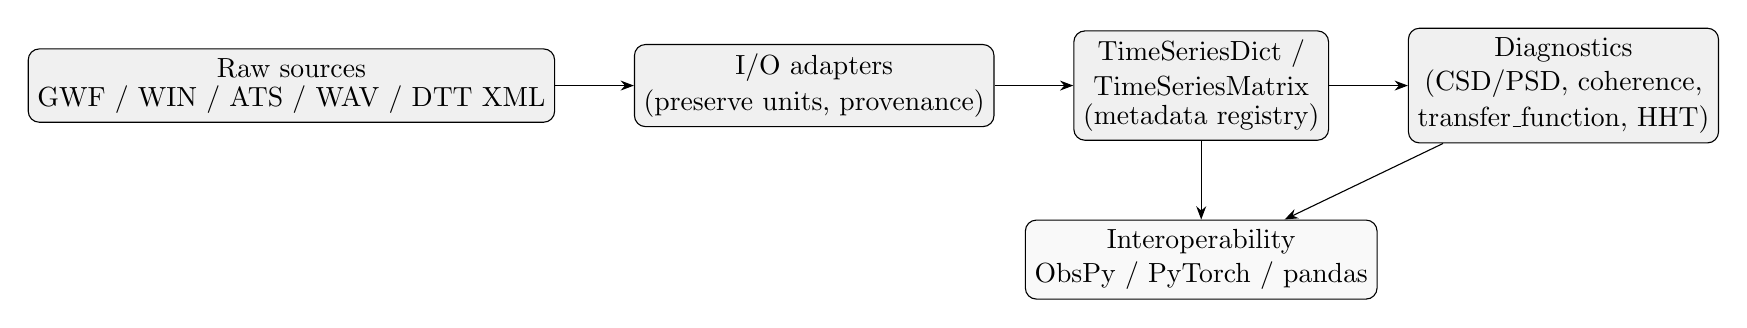
\begin{tikzpicture}[node distance=10mm,auto,>=Stealth]
    \node[draw, rectangle, rounded corners, fill=gray!12] (acq) {\shortstack{Raw sources\\GWF / WIN / ATS / WAV / DTT XML}};
    \node[draw, rectangle, rounded corners, right=of acq, fill=gray!12] (io) {\shortstack{I/O adapters\\(preserve units, provenance)}};
    \node[draw, rectangle, rounded corners, right=of io, fill=gray!12] (data) {\shortstack{TimeSeriesDict /\\TimeSeriesMatrix\\(metadata registry)}};
    \node[draw, rectangle, rounded corners, right=of data, fill=gray!12] (analysis) {\shortstack{Diagnostics\\(CSD/PSD, coherence,\\transfer\_function, HHT)}};
    \node[draw, rectangle, rounded corners, below=of data, fill=gray!5] (interop) {\shortstack{Interoperability\\ObsPy / PyTorch / pandas}};
    \draw[->] (acq) -- (io);
    \draw[->] (io) -- (data);
    \draw[->] (data) -- (analysis);
    \draw[->] (analysis) -- (interop);
    \draw[->] (data) -- (interop);
  \end{tikzpicture}
  \caption{High-level architecture of GWexpy.  The package performs deterministic I/O parsing into metadata-rich containers, enforces time-axis synchronization for matrix-level diagnostics, and provides interoperability helpers for cross-domain usage.  (For submission, this diagram is rendered from the repository's reproducible notebook.)}
  \label{fig:architecture}
\end{figure}

\subsection{Lossless cross-domain interoperability}
Conversions preserve metadata where target libraries permit.  Two examples:

\begin{itemize}
  \item \textbf{ObsPy:} Mapping of GWexpy channel metadata to ObsPy fields follows a documented mapping (channel $\to$ network/station/location/channel, sampling rate $\to$ stats.sampling\_rate, unit $\to$ stats.units with custom \texttt{stats['unit']} for non-standard unit objects).  The repository's documentation lists the mapping table and corner cases.
  \item \textbf{PyTorch:} Conversion to a \texttt{torch.Tensor} produces a contiguous numeric array while associating metadata as a companion Python object (a small dict or dataclass).  Round-trip helpers reconstruct \texttt{TimeSeriesMatrix} from a tensor + metadata object to ensure provenance.
\end{itemize}

% -------------------------
% DTT XML reader note
% -------------------------
\subsection{DTT XML reader: explicit product provenance}
\label{sec:dtt}
DTT XML exports (Diaggui / DTT) can contain heterogeneous measurement \emph{products} (transfer functions, coherence, PSD-like products).  GWexpy's DTT XML reader intentionally requires the user to specify the \texttt{products} argument to avoid ambiguous defaults and to make the analyst's intent explicit in the provenance record.  Example usage:

\begin{lstlisting}[caption={DTT XML: explicit product selection (public read API)}]
# recommended: explicit products argument
from gwexpy.timeseries import TimeSeriesDict, TimeSeriesMatrix

tsdict = TimeSeriesDict.read(
    source="measurement.xml",
    format="dttxml",
    channels=["PLANT:OUT", "PLANT:IN"],
    products=["tf"]  # explicit: 'tf' indicates transfer-function product
)

matrix = TimeSeriesMatrix.from_timeseries(list(tsdict.values()))
\end{lstlisting}

If \texttt{products} is omitted, the reader raises \texttt{ValueError("products must be specified for dttxml")}.  This decision is documented in the repository and is covered by unit tests that verify that the recorded provenance includes the original DTT XML node path and measurement parameters.

% -------------------------
% Illustrative examples
% -------------------------
\section{Illustrative examples}
The repository contains executable notebooks that reproduce the brief examples below.  These notebooks are validated in CI (see Section~\ref{sec:repro}).

\subsection{Example 1: DTT XML \textrightarrow{} transfer-function workflow}
This example shows a compact commissioning workflow that retains provenance and units.  The public API examples below are implemented in the repository; the Listing mirrors the tested notebook exactly.

\begin{lstlisting}[caption={DTT XML transfer-function workflow (public API)}]
from gwexpy.timeseries import TimeSeriesDict, TimeSeriesMatrix

# Read DTT XML with explicit product selection
tsdict = TimeSeriesDict.read(
    source="measurement.xml",
    format="dttxml",
    channels=["PLANT:OUT", "PLANT:IN"],
    products=["tf"]
)

# Build a synchronized multichannel object
matrix = TimeSeriesMatrix.from_timeseries(list(tsdict.values()))

# Estimate steady transfer function (Welch-based CSD/PSD)
# returns a FrequencySeries-like object with unit and provenance
tf = matrix.transfer_function(target="PLANT:OUT", reference="PLANT:IN", mode="steady")

# Plotting uses attached metadata to label axes automatically
tf.plot_bode()  # produces Bode magnitude/phase with channel labels and units
\end{lstlisting}

Figure~\ref{fig:bode} (generated by the manuscript notebook) shows a typical Bode plot produced by \texttt{plot\_bode()}; axis labels and legend entries are drawn from the metadata registry.

\begin{figure}[htbp]
  \centering
  \fbox{\parbox[c][6cm][c]{0.8\textwidth}{\centering External figure: Bode plot (generated by notebook)}}
  \caption{Example transfer-function (Bode) plot produced by \texttt{TimeSeriesMatrix.transfer\_function(...)}.  Axis labels, units and legend entries are provided automatically from preserved metadata.  (Figure reproduced by the repository notebook.)}
  \label{fig:bode}
\end{figure}

\subsection{Example 2: Heterogeneous format fusion \textrightarrow{} multichannel coherence ranking}
This example demonstrates fusion of multiple formats and coherence-based ranking:

\begin{lstlisting}[caption={Heterogeneous fusion and coherence-ranking}]
from gwexpy.timeseries import TimeSeries, TimeSeriesMatrix, TimeSeriesDict

t1 = TimeSeries.read(source="frame://ifo/frame", format="gwf", channels=["IFO:CH"])
t2 = TimeSeries.read(source="local_run.win", format="win", channels=["local_sensor_001"])
t3 = TimeSeries.read(source="recording.wav", format="wav", channels=["mic_01"])

matrix = TimeSeriesMatrix.from_timeseries([t1, t2, t3]).resample(rate=2048)

# Compute pairwise coherence relative to a target channel using Welch
# The returned object preserves channel metadata and offers ranking helpers
coh = matrix.coherence_ranking(target="IFO:CH", band=(10,100))
top_channels = coh.topk(n=3)  # top 3 channels most coherent with the target

# Visualize ranking: the plotting routine annotates by channel name and unit
coh.plot_ranked(top_k=3)
\end{lstlisting}

The internal implementation performs anti-aliasing resampling, Welch-based PSD/CSD estimation with documented windowing parameters, and parallelized pairwise CSD computations.  The method returns a metadata-rich summary object (see repository API docs).

% -------------------------
% Implementation details: signal processing & BruCo-style workflow
% -------------------------
\section{Implementation details}

\subsection{PSD/CSD, coherence and transfer estimation}
GWexpy's estimators are implemented using a Welch-based estimator for PSD/CSD with parameterizable FFT length, window type, and overlap.  Transfer-function estimation supports two modes:

\begin{itemize}
  \item \textbf{steady:} classical frequency-domain estimator using CSD/PSD (H1 = S\_{xy}/S\_{xx}) with optional regularization and uncertainty estimates computed from segment statistics (Welch).
  \item \textbf{transient:} short-time, FFT-windowed estimators designed for impulsive or non-stationary measurements; the package includes convenience wrappers to produce Bode-like visualizations for transient TF estimates.
\end{itemize}

All estimators produce objects carrying units (via \texttt{astropy.units}), measurement parameters (window length, overlap), and source provenance (input file/URI, DTT XML node path when applicable).

\subsection{BruCo-inspired automated noise-coupling workflows}
GWexpy implements an automated ranking workflow inspired by BruCo: for a target channel it computes pairwise coherence (or other coupling metrics) across a large set of auxiliary channels, aggregates per-frequency-band scores, and reports ranked suspect channels with per-score provenance.  The workflow supports:

\begin{itemize}
  \item Efficient computation by performing batched FFTs over the synchronized \texttt{TimeSeriesMatrix}, reducing I/O overhead compared with naive per-pair loops.
  \item Memory-efficient parallelization with chunked processing when the channel count is large.
  \item Post-processing to group alarms by physical origin (sensor families) using metadata tags.
\end{itemize}

Implementation details, performance microbenchmarks and example notebooks (N-channel scaling, benchmark against simple for-loop TimeSeriesDict approach) are included in the repository's supplement.

\subsection{HHT / EMD integration}
GWexpy provides wrappers to compute Empirical Mode Decomposition (EMD) and Hilbert--Huang spectra for non-stationary diagnostics.  The HHT output is represented as metadata-aware spectrogram-like objects that retain per-mode provenance and allow subsequent stacking, ranking and visualization without loss of unit information \cite{huang1998emd}.  Use cases include transient glitch morphology studies and time-localized coherence analysis.

% -------------------------
% Reproducibility and quality assurance
% -------------------------
\section{Reproducibility and testing}
\label{sec:repro}
GWexpy is distributed with:

\begin{itemize}
  \item A fully automated GitHub Actions CI pipeline that runs unit tests (pytest), notebook execution checks (nbmake) for the illustrative notebooks, style checks (ruff) and a GWpy-compatibility gate validating selected integration tests against the supported GWpy major version.
  \item Unit tests that assert metadata invariants (for example: metadata before/after conversion remains identical), coverage reporting, and examples that produce the manuscript figures.
  \item A release process: GitHub Release linked to a Zenodo archive (DOI to be added upon archival), containing the release tarball, example notebooks, environment specification (environment.yml and requirements.txt), and synthetic/anonymized example data sufficient to run the illustrative notebooks end-to-end.
\end{itemize}

These artifacts are linked from the Code metadata table below and from the repository README.

% -------------------------
% Impact
% -------------------------
\section{Impact}
GWexpy reduces the bookkeeping overhead of commissioning analyses by providing metadata-preserving multichannel containers and commissioning-tailored diagnostics.  Operationally, this shortens typical ad-hoc parsing workflows into concise, provenance-rich pipelines and reduces time spent debugging unit or timestamp mismatches.  Cross-domain benefits include enabling reproducible dataset creation for ML pipelines (PyTorch) and facilitating joint analyses with seismological toolchains (ObsPy).

% -------------------------
% Code metadata (SoftwareX C1--C9)
% -------------------------
\section*{Code metadata}
\begin{table}[htbp]
\centering
\begin{tabular}{|l|p{10cm}|}
\hline
\textbf{C1} & Current code version: \texttt{0.1.0} (release on GitHub; Zenodo DOI to be inserted after archival) \\\hline
\textbf{C2} & Permanent link to code/repository used for this code version: \url{https://github.com/tatsuki-washimi/gwexpy} \\\hline
\textbf{C3} & Permanent link to reproducible capsule: Zenodo DOI (to be provided at submission; the release contains environment.yml, notebooks and synthetic data) \\\hline
\textbf{C4} & Legal code license: MIT License (see \texttt{LICENSE}) \\\hline
\textbf{C5} & Code versioning system used: git (hosted on GitHub) \\\hline
\textbf{C6} & Software code languages, tools and services used: Python (primary). Key tools: pytest, nbmake, Sphinx (docs), GitHub Actions (CI). \\\hline
\textbf{C7} & Compilation requirements, operating environments and dependencies: Tested on Linux/macOS/Windows; Python $\ge$ 3.11. Core dependencies: \texttt{gwpy>=4.0.0}, \texttt{numpy>=1.21}, \texttt{scipy>=1.7}, \texttt{astropy>=5.0}, \texttt{pandas>=1.3}, \texttt{matplotlib>=3.5}. Optional extras: \texttt{obspy} (ObsPy interoperability), \texttt{torch} (PyTorch interoperability), \texttt{dttxml} (external DTT XML parser). See \texttt{pyproject.toml} for full spec. \\\hline
\textbf{C8} & If available, link to developer documentation/manual: \url{https://tatsuki-washimi.github.io/gwexpy/} (API docs, developer notes and tutorials) \\\hline
\textbf{C9} & Support email for questions: \texttt{tatsuki.washimi@nao.ac.jp} \\\hline
\end{tabular}
\end{table}

% -------------------------
% Acknowledgements
% -------------------------
\section*{Acknowledgements}
We thank the GWpy development community for designing an extensible foundation and commissioning teams at NAOJ for feedback during GWexpy's development.  This work was informed by BruCo-style workflows and by public toolchains for detector characterization.

% -------------------------
% References
% -------------------------
\begin{thebibliography}{99}

\bibitem{gwpy}
D. M. Macleod, J. S. Areeda, S. B. Coughlin, T. J. Massinger, and A. L. Urban,
``GWpy: A Python package for gravitational-wave astrophysics,''
\textit{SoftwareX} \textbf{13}, 100657 (2021). \doi{10.1016/j.softx.2021.100657}

\bibitem{huang1998emd}
N. E. Huang, Z. Shen, S. R. Long, M. C. Wu, H. H. Shih, Q. Zheng, N.-C. Yen, C.-C. Tung, and H.-H. Liu,
``The empirical mode decomposition and the Hilbert spectrum for nonlinear and non-stationary time series analysis,''
\textit{Proc. R. Soc. A} \textbf{454}, 903--995 (1998). \doi{10.1098/rspa.1998.0193}

\bibitem{vajente2022datamining}
G. Vajente,
``Data mining and machine learning improve gravitational-wave detector sensitivity,''
\textit{Phys. Rev. D} \textbf{105}, 102005 (2022). \doi{10.1103/PhysRevD.105.102005}

\bibitem{ligo_t1300432}
LSC--Virgo Collaboration, ``The 2013--2014 data analysis, software and computing, detector characterization white paper,'' LIGO Technical Note LIGO-T1300432-v2 (2013). \url{https://dcc.ligo.org/LIGO-T1300432/public}

\bibitem{ligo_transient_noise_2016}
LIGO Scientific Collaboration and Virgo Collaboration,
``Characterization of transient noise in Advanced LIGO relevant to gravitational wave signal GW150914,''
\textit{Class. Quantum Grav.} \textbf{33}, 134001 (2016). \doi{10.1088/0264-9381/33/13/134001}

\bibitem{beyreuther2010obspy}
M. Beyreuther, R. Barsch, L. Krischer, T. Megies, Y. Behr, and J. Wassermann,
``ObsPy: A Python Toolbox for Seismology,''
\textit{Seismol. Res. Lett.} \textbf{81}(3), 530--533 (2010). \doi{10.1785/gssrl.81.3.530}

\bibitem{paszke2019pytorch}
A. Paszke et al., ``PyTorch: An Imperative Style, High-Performance Deep Learning Library,'' in \textit{Advances in Neural Information Processing Systems 32 (NeurIPS 2019)}, 8024--8035 (2019).

\end{thebibliography}

\end{document}